\section{Results: Default Parameters}


After implementing the described environment and controllers with all specified parameters, the following results were obtained for the
baseline controllers in the mixed near-congested/congested traffic scenario.

\subsection{Comparison: Replication vs Paper Baselines}

\subsubsection{Mixed Traffic Scenario}

\begin{table}[H]
\centering
\small
\caption{Replication vs Paper Values (Mixed Traffic, Default Scenario)}
\begin{tabular}{l c c c}
\toprule
\textbf{Metric} & \textbf{Replication} & \textbf{Paper} & \textbf{Deviation} \\
\midrule
\multicolumn{4}{l}{\textit{ALINEA}} \\
\midrule
Throughput (veh/h)       & 3843.66 & 3664.71 & +4.88\% \\
Speed (m/s)              & 11.87   & 12.42   & $-$4.43\% \\
Stops per Vehicle        & 0.86    & 11.33   & $-$92.41\% \\
Fuel Efficiency (mpg)    & 19.47   & 17.00   & +14.53\% \\
CO$_2$ Emissions (g/mi)  & 479.55  & 512.99  & $-$6.52\% \\
NO$_x$ Emissions (mg/mi) & 194.11  & 208.00  & $-$6.68\% \\
\midrule
\multicolumn{4}{l}{\textit{Fixed}} \\
\midrule
Throughput (veh/h)       & 3846.35 & 3493.46 & +10.10\% \\
Speed (m/s)              & 12.56   & 14.18   & $-$11.42\% \\
Stops per Vehicle        & 0.89    & 3.62    & $-$75.41\% \\
Fuel Efficiency (mpg)    & 19.12   & 18.26   & +4.71\% \\
CO$_2$ Emissions (g/mi)  & 499.82  & 481.71  & +3.76\% \\
NO$_x$ Emissions (mg/mi) & 203.32  & 195.00  & +4.27\% \\
\midrule
\multicolumn{4}{l}{\textit{No Ramp Meter}} \\
\midrule
Throughput (veh/h)       & 3855.16 & 3664.71 & +5.20\% \\
Speed (m/s)              & 12.49   & 11.05   & +13.03\% \\
Stops per Vehicle        & 0.69    & 18.89   & $-$96.35\% \\
Fuel Efficiency (mpg)    & 20.41   & 16.01   & +27.48\% \\
CO$_2$ Emissions (g/mi)  & 454.00  & 548.61  & $-$17.25\% \\
NO$_x$ Emissions (mg/mi) & 182.31  & 226.09  & $-$19.36\% \\
\bottomrule
\end{tabular}
\end{table}

With the default parameters, the two metrics we identified as most important, traffic throughput 
and average vehicle speed, show notable deviations from the values reported in the original paper.
The deviation in average vehicle speed of up to 13.03\% in the no ramp meter scenario was particularly pronounced and motivated the parameter tuning presented in the next section. 
For compactness, the remaining plots and tables for the default-parameter setup are provided in the appendix.



\section{Results: Tuned Parameters}

Since the metrics reported by the original work could not be reproduced with the original parameter setting, we empirically tuned the baseline controllers in order to obtain more accurate values for traffic throughput (veh/h) and average vehicle speed (m/s) in the mixed near-congested/congested traffic scenario.

After extensive experimentation and iterative refinement, the following adjustments were introduced (referred to as the \textit{Tuned Setup} in the remainder of this paper):

\begin{itemize}
\item For the vehicle type, the minimum time headway between two consecutive vehicles was increased from the default value of $\tau = 1.00$s to $\tau = 1.04$s. A larger value of $\tau$ results in a slightly more cautious car-following behaviour and therefore slightly reduces traffic throughput and speed.
\item For the fixed-time controller, the cycle length was extended from 4s to 16s, consisting of a 15s red phase and a 1s green phase. Consequently, fewer vehicles were admitted to the freeway per simulation episode, which restricted the on-ramp inflow and therefore reduced congestion at the merging area, leading to higher average vehicle speeds.
\item For the ALINEA controller, all original parameters were kept unchanged. However, instead of deriving the two variables $q_\text{freeway}$ and $q_\text{ramp}$ from a single snapshot of the most recent simulation step, both were averaged over a sliding window of ten simulation steps. This reduced measurement noise and yielded a more stable control signal, which in our experiments led to a slight increase in both traffic throughput and average vehicle speed.
\item The RL controllers themselves were left unchanged but retrained on the tuned vehicle type with $\tau = 1.04$s.
\end{itemize}

The obtained values for the baseline controllers are compared to the reported values in the original study in the table below.

\subsection{Comparison: Replication vs Paper Baselines}

\subsubsection{Mixed Traffic Scenario}

\begin{table}[H]
\centering
\small
\caption{Replication vs Paper Values (Mixed Traffic, Tuned Scenario)}
\begin{tabular}{l c c c}
\toprule
\textbf{Metric} & \textbf{Replication} & \textbf{Paper} & \textbf{Deviation} \\
\midrule
\multicolumn{4}{l}{\textit{No Ramp Meter}} \\
\midrule
Throughput (veh/h)       & 3840.42 & 3664.71 & +4.79\% \\
Speed (m/s)              & 11.33   & 11.05   & +2.53\% \\
Stops per Vehicle        & 0.83    & 18.89   & $-$95.61\% \\
Fuel Efficiency (mpg)    & 19.29   & 16.01   & +20.49\% \\
CO$_2$ Emissions (g/mi)  & 479.98  & 548.61  & $-$12.51\% \\
NO$_x$ Emissions (mg/mi) & 194.38  & 226.09  & $-$14.03\% \\
\midrule
\multicolumn{4}{l}{\textit{Fixed}} \\
\midrule
Throughput (veh/h)       & 3849.59 & 3493.46 & +10.19\% \\
Speed (m/s)              & 14.06   & 14.18   & $-$0.85\% \\
Stops per Vehicle        & 1.17    & 3.62    & $-$67.68\% \\
Fuel Efficiency (mpg)    & 19.16   & 18.26   & +4.93\% \\
CO$_2$ Emissions (g/mi)  & 572.45  & 481.71  & +18.84\% \\
NO$_x$ Emissions (mg/mi) & 236.62  & 195.00  & +21.34\% \\
\midrule
\multicolumn{4}{l}{\textit{ALINEA}} \\
\midrule
Throughput (veh/h)       & 3851.75 & 3664.71 & +5.10\% \\
Speed (m/s)              & 12.61   & 12.42   & +1.53\% \\
Stops per Vehicle        & 1.04    & 11.33   & $-$90.82\% \\
Fuel Efficiency (mpg)    & 19.00   & 17.00   & +11.76\% \\
CO$_2$ Emissions (g/mi)  & 505.95  & 512.99  & $-$1.37\% \\
NO$_x$ Emissions (mg/mi) & 206.10  & 208.00  & $-$0.91\% \\
\bottomrule
\end{tabular}
\end{table}

While the deviation in the traffic throughput remained similar to the default configuration, the deviation in average vehicle speed could be decreased to at most 2.53\% across all baseline controllers.

The same comparison for the extreme traffic scenario is shown below.

\subsubsection{Extreme Traffic Scenario}

\begin{table}[H]
\centering
\small
\caption{Replication vs Paper Values (Extreme Traffic, Tuned Scenario)}
\begin{tabular}{l c c c}
\toprule
\textbf{Metric} & \textbf{Replication} & \textbf{Paper} & \textbf{Deviation} \\
\midrule
\multicolumn{4}{l}{\textit{ALINEA}} \\
\midrule
Throughput (veh/h)       & 4421.60 & 3790.29 & +16.66\% \\
Speed (m/s)              & 6.87    & 10.62   & $-$35.31\% \\
Stops per Vehicle        & 4.75    & 11.73   & $-$59.51\% \\
Fuel Efficiency (mpg)    & 11.30   & 16.83   & $-$32.86\% \\
CO$_2$ Emissions (g/mi)  & 874.53  & 518.52  & +68.66\% \\
NO$_x$ Emissions (mg/mi) & 374.56  & 212.66  & +76.13\% \\
\midrule
\multicolumn{4}{l}{\textit{Fixed}} \\
\midrule
Throughput (veh/h)       & 4419.80 & 3648.60 & +21.14\% \\
Speed (m/s)              & 7.12    & 9.57    & $-$25.60\% \\
Stops per Vehicle        & 4.50    & 7.18    & $-$37.33\% \\
Fuel Efficiency (mpg)    & 11.43   & 15.82   & $-$27.75\% \\
CO$_2$ Emissions (g/mi)  & 926.45  & 552.63  & +67.64\% \\
NO$_x$ Emissions (mg/mi) & 398.49  & 227.03  & +75.52\% \\
\midrule
\multicolumn{4}{l}{\textit{No Ramp Meter}} \\
\midrule
Throughput (veh/h)       & 4420.52 & 3683.02 & +20.02\% \\
Speed (m/s)              & 6.17    & 9.45    & $-$34.71\% \\
Stops per Vehicle        & 4.90    & 25.42   & $-$80.72\% \\
Fuel Efficiency (mpg)    & 11.16   & 15.25   & $-$26.82\% \\
CO$_2$ Emissions (g/mi)  & 881.45  & 575.34  & +53.21\% \\
NO$_x$ Emissions (mg/mi) & 377.69  & 236.62  & +59.62\% \\
\bottomrule
\end{tabular}
\end{table}

Since the parameters were tuned specifically to improve the match in the mixed near-congested/congested traffic scenario, the deviations in the extreme traffic scenario did not improve accordingly. 
However, for completeness, we still report the obtained values for the baseline controllers in the extreme traffic conditions in 
the above table. 
\medskip

Having established more accurate baseline values in the mixed traffic scenario, we now turn to the three
reinforcement learning based controllers. In line with the original study, all three RL agents were trained exclusively on mixed near-congested and congested traffic conditions. The extremely congested case is used solely for testing the trained policies. We first examine their training convergence before comparing their final performance against the baselines introduced above.

\subsection{Convergence Analysis of Reinforcement Learning Controllers}

%------------------------------------------------
% Ape-X DQN
%------------------------------------------------

\paragraph{Ape-X DQN}

\begin{figure}[H]
  \centering
  \begin{minipage}[t]{0.48\linewidth}
    \centering
    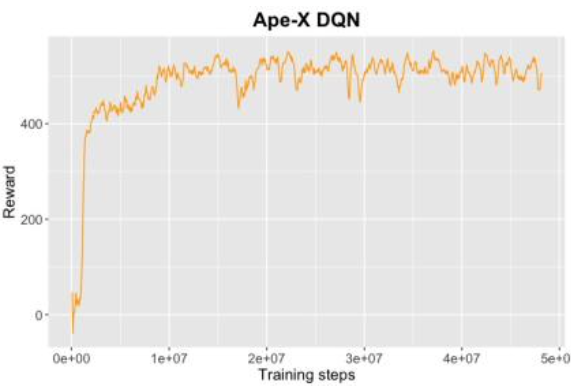
\includegraphics[width=\linewidth]{figures/results/Tuned/RL_convergence/original/apexdqn_reward.png}
  \end{minipage}
  \hfill
  \begin{minipage}[t]{0.48\linewidth}
    \centering
    
\includegraphics[width=\linewidth]{figures/results/Tuned/RL_convergence/replication/apexdqn_reward.png}
  \end{minipage}
  \caption{Ape-X DQN training convergence: original (left) vs.\ replication (right).}
\end{figure}

While the reward curve of Ape-X DQN in the original work shows a clear convergence
trend after approximately 20 million training steps, the replicated curve fails to reach a stable convergence
trend, ending approximately 100 reward points below the original. 


%------------------------------------------------
% PPO
%------------------------------------------------

\paragraph{PPO}

\begin{figure}[H]
  \centering
  \begin{minipage}[t]{0.48\linewidth}
    \centering
    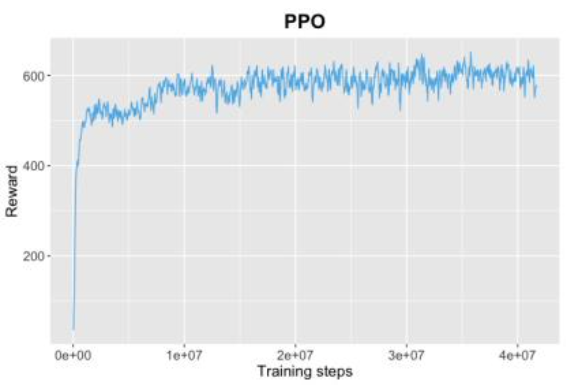
\includegraphics[width=\linewidth]{figures/results/Tuned/RL_convergence/original/ppo_reward.png}
  \end{minipage}
  \hfill
  \begin{minipage}[t]{0.48\linewidth}
    \centering
    
\includegraphics[width=\linewidth]{figures/results/Tuned/RL_convergence/replication/ppo_reward.png}
  \end{minipage}
  \caption{PPO training convergence: original (left) vs.\ replication (right).}
\end{figure}

PPO shows a comparable pattern: The replicated reward curve ends
roughly 200 points below the value observed in the original reward curve.


%------------------------------------------------
% A3C
%------------------------------------------------

\paragraph{A3C}

\begin{figure}[H]
  \centering
  \begin{minipage}[t]{0.48\linewidth}
    \centering
    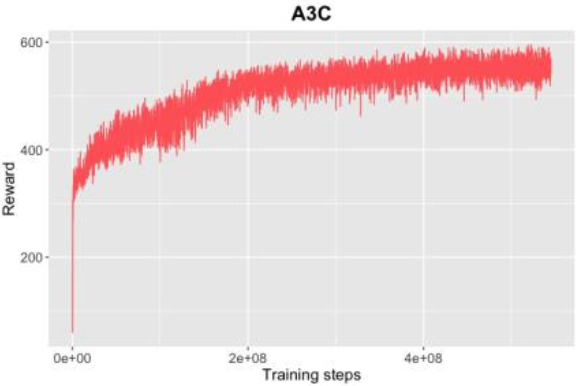
\includegraphics[width=\linewidth]{figures/results/Tuned/RL_convergence/original/a3c_reward.png}
  \end{minipage}
  \hfill
  \begin{minipage}[t]{0.48\linewidth}
    \centering
    
\includegraphics[width=\linewidth]{figures/results/Tuned/RL_convergence/replication/a3c_reward.png}
  \end{minipage}
  \caption{A3C training convergence: original (left) vs.\ replication (right).}
\end{figure}

In the original work, A3C converges after 300 million training steps, reaching about 550 reward points at the end of training. In our replication, the reward curve plateaus after around 100 million steps and continues to oscillate between approximately 330--410 reward points.
\medskip
Note that the y-axis of the replication plots is auto-scaled to the value range observed during training and is not anchored at zero, in order to better highlight the shape of the learning curve.
\medskip
The following section evaluates the final performances of the RL controllers and compares them to those of the baseline controllers in a boxplot illustration.

\subsection{Boxplots: RL vs Baselines}

\subsubsection{Mixed Traffic Scenario}

\begin{figure}[H]
  \centering
  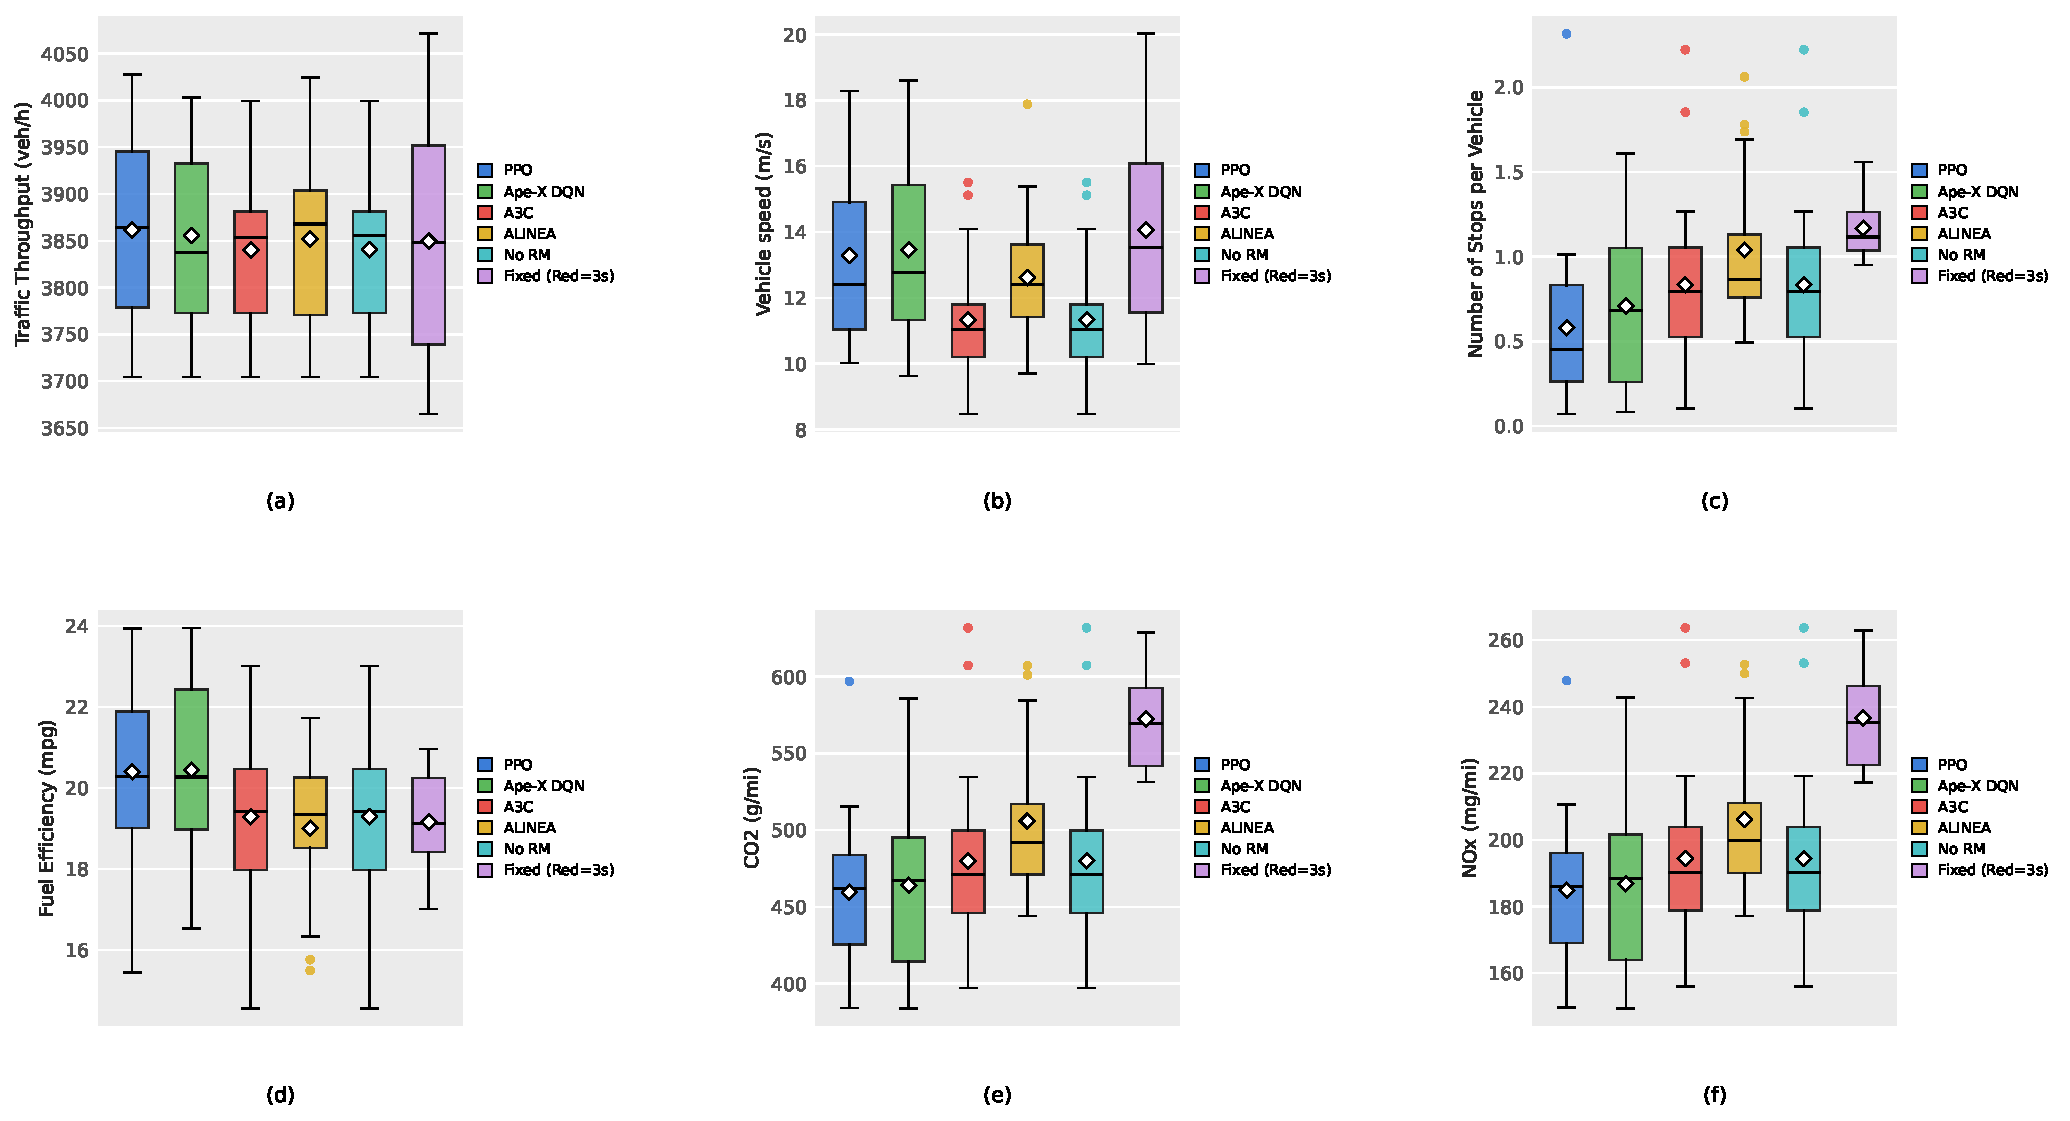
\includegraphics[width=\linewidth]{figures/results/Tuned/Mixed/boxplots_mixed.pdf}
  \caption{Performance metrics for the mixed traffic scenario. (a) Traffic Throughput (veh/h), (b) Average Vehicle Speed (m/s), (c) Number of Stops per Vehicle, (d) Fuel Efficiency (mpg), (e) CO$_2$ Emissions (g/mi), (f) NO$_x$ Emissions (mg/mi).}
\end{figure}

While Hou et al. report that PPO outperforms the other two RL algorithms in each of the six metrics, our results show that PPO has a slightly lower average vehicle speed and slightly lower fuel efficiency than Ape-X DQN. Therefore, we cannot confirm this claim. 
Generally, all six controllers show similar performance in traffic throughput, number of stops per vehicle and fuel efficiency. The large performance gap between the RL controllers and the baseline controllers that can be observed in Figure 4 (for example average speeds of around 18--20 m/s, significantly higher fuel efficiency or a lower number of stops for the RL controllers) of the original paper could not be reproduced. 
Another notable observation is that A3C performs almost identically to the no ramp metering case, suggesting that the learned policy mostly keeps the ramp meter green and switches to red only a few times per episode.

\subsubsection{Extreme Traffic Scenario}

\begin{figure}[H]
  \centering
  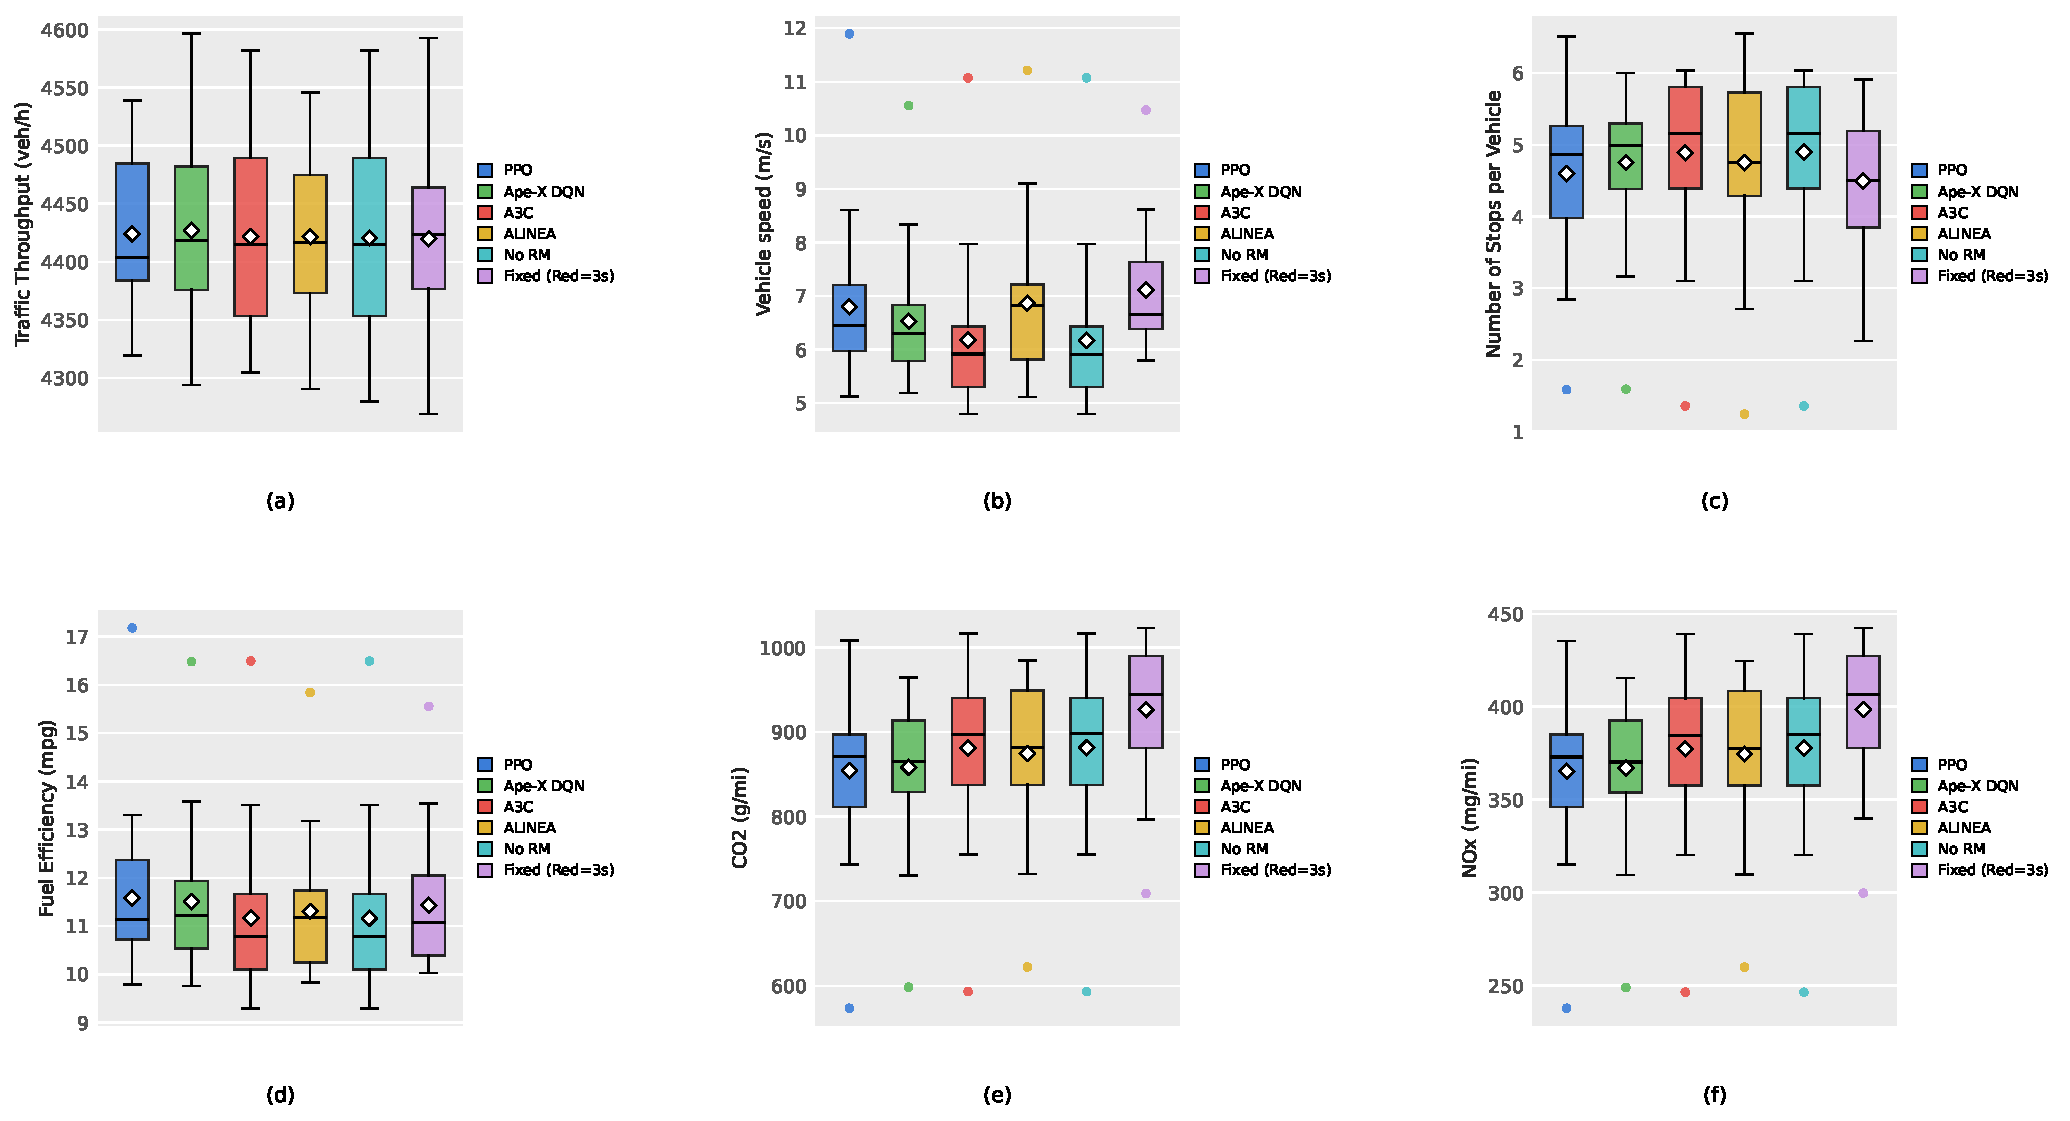
\includegraphics[width=\linewidth]{figures/results/Tuned/Extreme/boxplots_extreme.pdf}
  \caption{Performance metrics for the extreme traffic scenario. (a) Traffic Throughput (veh/h), (b) Average Vehicle Speed (m/s), (c) Number of Stops per Vehicle, (d) Fuel Efficiency (mpg), (e) CO$_2$ Emissions (g/mi), (f) NO$_x$ Emissions (mg/mi).}
\end{figure}

In the extreme traffic scenario, the three RL-based controllers as well as the baseline controllers result in very similar performance across all six metrics. 
The means of the throughput are almost identical, whereas in Figure 5 of the original paper PPO and A3C 
clearly outperform all other controllers in throughput and speed. In our reproduction, no clear winner 
can be identified and notably the fixed-time controller achieves the highest average vehicle speed.
In this scenario, A3C again collapses to a behaviour similar to the no ramp metering case.
Even though PPO has the highest fuel efficiency on average and the lowest CO$_2$ and NO$_x$ emissions, the superiority of PPO in all metrics that is claimed in the paper could not be confirmed. 

\medskip

In the next section, we compare the performance of the RL controller average to the baselines across all metrics and show the percentage deviation of the RL controller average to the baseline values. 

\subsection{Performance Comparison: RL vs Baselines}


\subsubsection{Mixed Traffic Scenario}

\begin{table}[H]
\centering
\small
\caption{RL Average vs Baseline Controllers: Mixed Traffic Conditions (Tuned Parameters)}
\begin{tabular}{l c c c c}
\toprule
\multirow{2}{*}{\textbf{Performance Metric}} & \multirow{2}{*}{\textbf{RL Average}} & \multicolumn{3}{c}{\textbf{Changes Compared with Baseline}} \\
\cmidrule(lr){3-5}
 & & \textbf{ALINEA} & \textbf{No Ramp Meter} & \textbf{Fixed} \\
\midrule
Traffic throughput (vph)                      & 3{,}852.47 & +0.02\% & +0.31\%  & +0.07\%  \\
Average vehicle speed (m/s)                   & 12.69      & +0.63\% & +12.00\% & $-$9.74\%  \\
Average number of stops per vehicle           & 0.71       & $-$31.73\% & $-$14.46\% & $-$39.32\% \\
Average vehicle fuel efficiency (mpg)         & 20.04      & +5.47\% & +3.89\%  & +4.59\%  \\
Average CO$_2$ emissions per vehicle (g/mi)   & 467.92     & $-$7.52\% & $-$2.51\%  & $-$18.26\% \\
Average NO$_x$ emissions per vehicle (mg/mi)  & 188.71     & $-$8.44\% & $-$2.92\%  & $-$20.25\% \\
\bottomrule
\end{tabular}
\end{table}

\begin{table}[H]
\centering
\small
\caption{RL Average vs Baseline Controllers: Mixed Traffic Conditions (Original Paper)}
\begin{tabular}{l c c c c}
\toprule
\multirow{2}{*}{\textbf{Performance Metric}} & \multirow{2}{*}{\textbf{RL Average}} & \multicolumn{3}{c}{\textbf{Changes Compared with Baseline}} \\
\cmidrule(lr){3-5}
 & & \textbf{ALINEA} & \textbf{No Ramp Meter} & \textbf{Fixed} \\
\midrule
Traffic throughput (vph)                      & 3{,}738 & +2\%   & +2\%   & +7\%   \\
Average vehicle speed (m/s)                   & 19.0    & +53\%  & +72\%  & +34\%  \\
Average number of stops per vehicle           & 1.7     & $-$85\% & $-$91\% & $-$53\% \\
Average vehicle fuel efficiency (mpg)         & 22.1    & +30\%  & +38\%  & +21\%  \\
Average CO$_2$ emissions per vehicle (g/mi)   & 395     & $-$23\% & $-$28\% & $-$18\% \\
Average NO$_x$ emissions per vehicle (mg/mi)  & 156     & $-$25\% & $-$31\% & $-$20\% \\
\bottomrule
\end{tabular}
\end{table}

The reported superiority of the RL controllers across the given metrics in the table could not be confirmed. 
For traffic throughput, the RL average is very similar to the baselines, with a maximum increase of 0.31\% compared to the no ramp meter controller. 
Even though the RL average outperforms ALINEA and no ramp metering in terms of average vehicle speed, it is surprisingly about 10\% slower than the fixed-time controller. 
While the RL average clearly outperforms the baseline controllers regarding average number of stops per vehicle, the reported decrease is still significantly higher in the original paper. 
For the last three metrics (average vehicle fuel efficiency, average CO$_2$ emissions per vehicle and average NO$_x$ emissions per vehicle), the reproduction results confirm the improvement of the RL average, but not in the magnitude that is reported by Hou et al. 

\subsubsection{Extreme Traffic Scenario}

\begin{table}[H]
\centering
\small
\caption{RL Average vs Baseline Controllers: Extreme Traffic Conditions (Tuned Parameters)}
\begin{tabular}{l c c c c}
\toprule
\multirow{2}{*}{\textbf{Performance Metric}} & \multirow{2}{*}{\textbf{RL Average}} & \multicolumn{3}{c}{\textbf{Changes Compared with Baseline}} \\
\cmidrule(lr){3-5}
 & & \textbf{ALINEA} & \textbf{No Ramp Meter} & \textbf{Fixed} \\
\midrule
Traffic throughput (vph)                      & 4{,}424.36 & +0.06\%    & +0.09\%   & +0.10\%   \\
Average vehicle speed (m/s)                   & 6.50       & $-$5.39\%  & +5.35\%   & $-$8.71\% \\
Average number of stops per vehicle           & 4.75       & +0.00\%    & $-$3.06\% & +5.56\%   \\
Average vehicle fuel efficiency (mpg)         & 11.42      & +1.06\%    & +2.33\%   & $-$0.09\% \\
Average CO$_2$ emissions per vehicle (g/mi)   & 864.45     & $-$1.15\%  & $-$1.93\% & $-$6.69\% \\
Average NO$_x$ emissions per vehicle (mg/mi)  & 369.96     & $-$1.23\%  & $-$2.05\% & $-$7.16\% \\
\bottomrule
\end{tabular}
\end{table}

\begin{table}[H]
\centering
\small
\caption{RL Average vs Baseline Controllers: Extreme Traffic Conditions (Original Paper)}
\begin{tabular}{l c c c c}
\toprule
\multirow{2}{*}{\textbf{Performance Metric}} & \multirow{2}{*}{\textbf{RL Average}} & \multicolumn{3}{c}{\textbf{Changes Compared with Baseline}} \\
\cmidrule(lr){3-5}
 & & \textbf{ALINEA} & \textbf{No Ramp Meter} & \textbf{Fixed} \\
\midrule
Traffic throughput (vph)                      & 3{,}904 & +3\%   & +6\%   & +7\%   \\
Average vehicle speed (m/s)                   & 15.4    & +45\%  & +63\%  & +61\%  \\
Average number of stops per vehicle           & 6.1     & $-$48\% & $-$76\% & $-$15\% \\
Average vehicle fuel efficiency (mpg)         & 21.2    & +26\%  & +39\%  & +34\%  \\
Average CO$_2$ emissions per vehicle (g/mi)   & 420     & $-$19\% & $-$27\% & $-$24\% \\
Average NO$_x$ emissions per vehicle (mg/mi)  & 168     & $-$21\% & $-$29\% & $-$26\% \\
\bottomrule
\end{tabular}
\end{table}


For the extreme traffic scenario, the RL average shows very similar performance to the baseline controllers across all six metrics.
While traffic throughput is almost identical across all controllers, we could not confirm the reported speed increase of 45--63\% for the RL average. In fact, the RL average was even slower than both ALINEA and the fixed-time controller. 
Furthermore, the paper reports a significant decrease in CO$_2$ and NO$_x$ emissions, average number of stops per vehicle and a substantial increase in fuel efficiency for the RL average, which we could not confirm in our reproduction. 
\medskip
In the last section of the results, we analyse the speed across the freeway.
In order to get these plots, we divide the freeway mainline (Seg. 1 - 8, excluding the on-ramp) into 5-meter bins, compute for each bin the mean speed across all simulation steps and evaluation episodes per controller, and render the result using a colormap (0–30 m/s), where brighter colors indicate higher speeds and the red rectangle marks the merging area (Seg. 6).

\subsection{Spatial Speed Analysis}

\subsubsection{Mixed Traffic Scenario}

\begin{figure}[H]
  \centering
  \begin{minipage}[t]{0.48\linewidth}
    \centering
    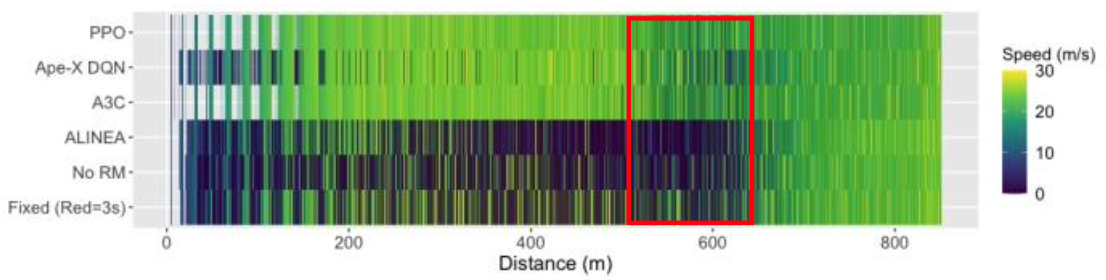
\includegraphics[width=\linewidth]{figures/results/Tuned/Mixed/speedmap_mixed_original.png}
  \end{minipage}
  \hfill
  \begin{minipage}[t]{0.48\linewidth}
    \centering
    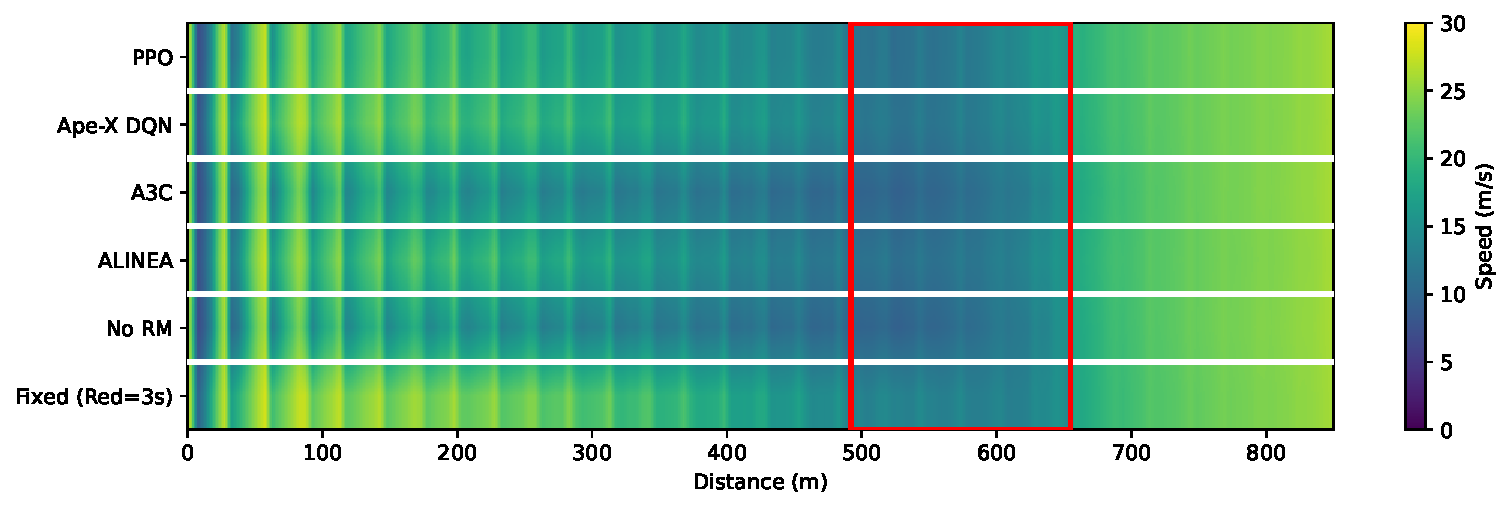
\includegraphics[width=\linewidth]{figures/results/Tuned/Mixed/speedmap_mixed.pdf}
  \end{minipage}
  \caption{Spatial speed distribution for the mixed traffic scenario: original (left) vs.\ replication (right).}
\end{figure}


While the original paper shows noticeably darker colors in the first 600\,m of the freeway for the baseline controllers and predominantly green colors for the RL controllers, indicating a significant speed increase, the reproduced speedmaps display a similar color distribution across all controllers. This suggests that the speed improvement attributed to the RL controllers could not be reproduced.


\subsubsection{Extreme Traffic Scenario}

\begin{figure}[H]
  \centering
  \begin{minipage}[t]{0.48\linewidth}
    \centering
    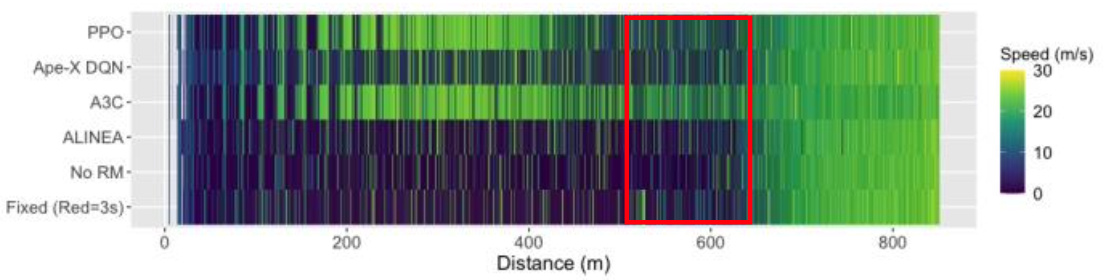
\includegraphics[width=\linewidth]{figures/results/Tuned/Extreme/speedmap_extreme_original.png}
  \end{minipage}
  \hfill
  \begin{minipage}[t]{0.48\linewidth}
    \centering
    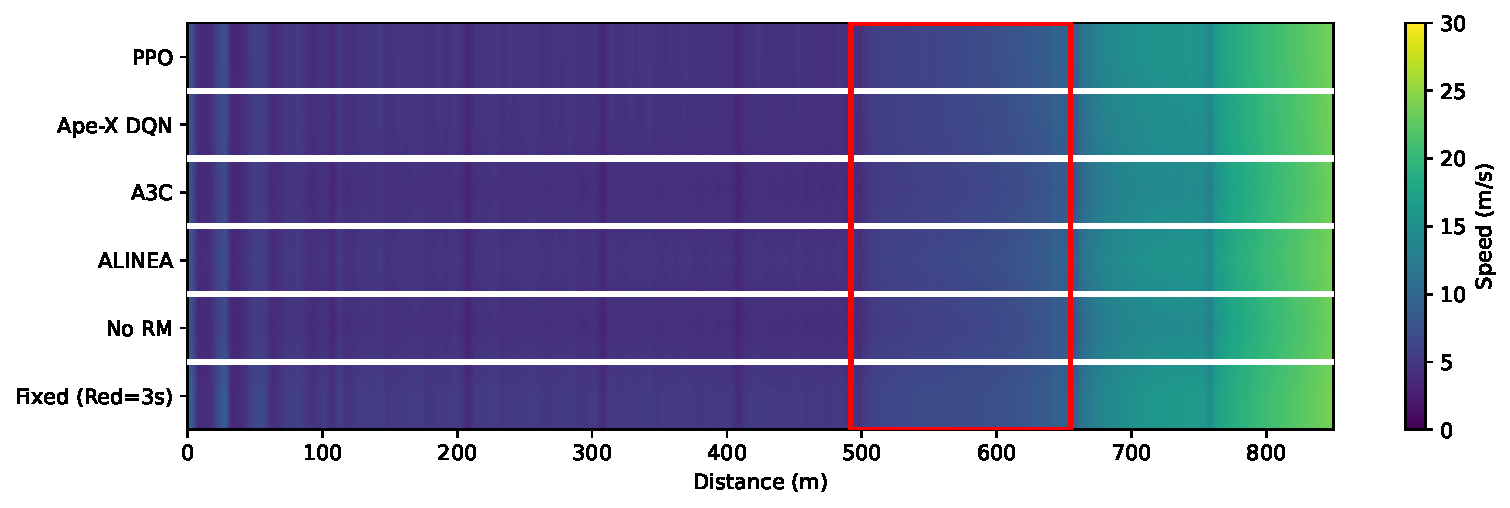
\includegraphics[width=\linewidth]{figures/results/Tuned/Extreme/speedmap_extreme.pdf}
  \end{minipage}
  \caption{Spatial speed distribution for the extreme traffic scenario: original (left) vs.\ replication (right).}
\end{figure}

Whereas in the original speedmap one can clearly see green colors for the RL controllers, especially PPO and A3C, in the range between 200\,m and 600\,m, the reproduced speedmap is colored completely blue for all controllers in the said interval. This clearly reveals that the average vehicle speed across the freeway could not be increased by RL-based controllers in the extreme traffic scenario, contrary to the claim of the original paper. 
